% Quick start guide
\documentclass[10pt]{beamer}

\usepackage{mathtools}

% Title page details
\title{Stochastic Calculus}
\author{Kellen Kanarios}
\institute{University of Michigan}
\date{\today}

\begin{document}

\begin{frame}
% Print the title page as the first slide
\titlepage
\end{frame}

\begin{frame}[t]
  \frametitle{Background}
  \begin{onlyenv}<1-9>
    \begin{definition}
      A real-valued random variable $X$ is a mapping $X : \Omega \to \mathbb{R}$. Here, $\Omega$ is the \textbf{sample space} and $\mathbb{P}$ is the measure of the \textbf{probability space}, such that $\mathbb{P}(\Omega) = 1$.
    \end{definition}
  \end{onlyenv}
  \begin{onlyenv}<2-5>
      \begin{block}{Note}
        Intuition for a \textbf{measure}:
        \begin{enumerate}
          \item <3-> In $\mathbb{R}$: length,
          \item <4-> In $\mathbb{R}^2$: area,
          \item <5-> In $\mathbb{R}^3$: volume.
        \end{enumerate}
      \end{block}
  \end{onlyenv}
  \begin{onlyenv}<6-9>
      \begin{block}{Definition translated into english}
        \begin{enumerate}
          \item<7->
            Unbeknownst to us, someone chooses a random $\omega \in \Omega$. Then we see the $X(\omega) \in \mathbb{R}$.
          \item<8->
            We cannot see the corresponding $\omega \in \Omega$, but the $X(\omega) \in \mathbb{R}$ gives us partial information about $\omega$.
          \item<9-> $\mathbb{P}$ tells us how likely subsets $A \subseteq \Omega$ are to occur.
        \end{enumerate}
      \end{block}
  \end{onlyenv}
  \begin{onlyenv}<10>
    \begin{example}
      Consider the case where you flip a coin. Using our previous definition, this could be described as $\Omega = \{\text{heads}, \text{tails}\}$ and \\
      \vskip 5pt
      $X(\omega) = \begin{cases}
        1, &\text{ if }\omega = \text{heads}\\
        -1, &\text{ if }\omega = \text{tails}\\
      \end{cases}$ \hspace*{10mm} where $\omega \in \Omega$. \\
      \vskip 5pt
      This would yield the familiar notation of $\mathbb{P}(X = 1) = .5$ and $\mathbb{P}(X = -1) = .5$ for a fair coin.
    \end{example} 
    \end{onlyenv}
    \begin{onlyenv}<11->
      \begin{definition}
        A \textbf{stochastic process} is a family of random variables indexed by a time parameter $t \geq 0$.
      \end{definition}
    \end{onlyenv}
    \begin{onlyenv}<12->
      \begin{example}
        A sequence of coin flips. At each time $t$ your process corresponds to a random variable (aka coinflip) $X_t$.
      \end{example}
    \end{onlyenv}
\end{frame}


\begin{frame}[t]
  \frametitle{Wiener Process}
  \begin{onlyenv}<1-5>
  \begin{definition}
    A stochastic process $W$ is called a \textbf{Wiener process} if the follow conditions hold:
    \begin{enumerate}
      \item<2-> $W_0 = 0$,
      \item<3-> The process $W$ has independent increments,
      \item<4->
          For $s < t$ the random variable $W_t - W_s$ has the Gaussian distribution $\mathcal{N}(0,t-s)$,
          \begin{figure}
            \centering
            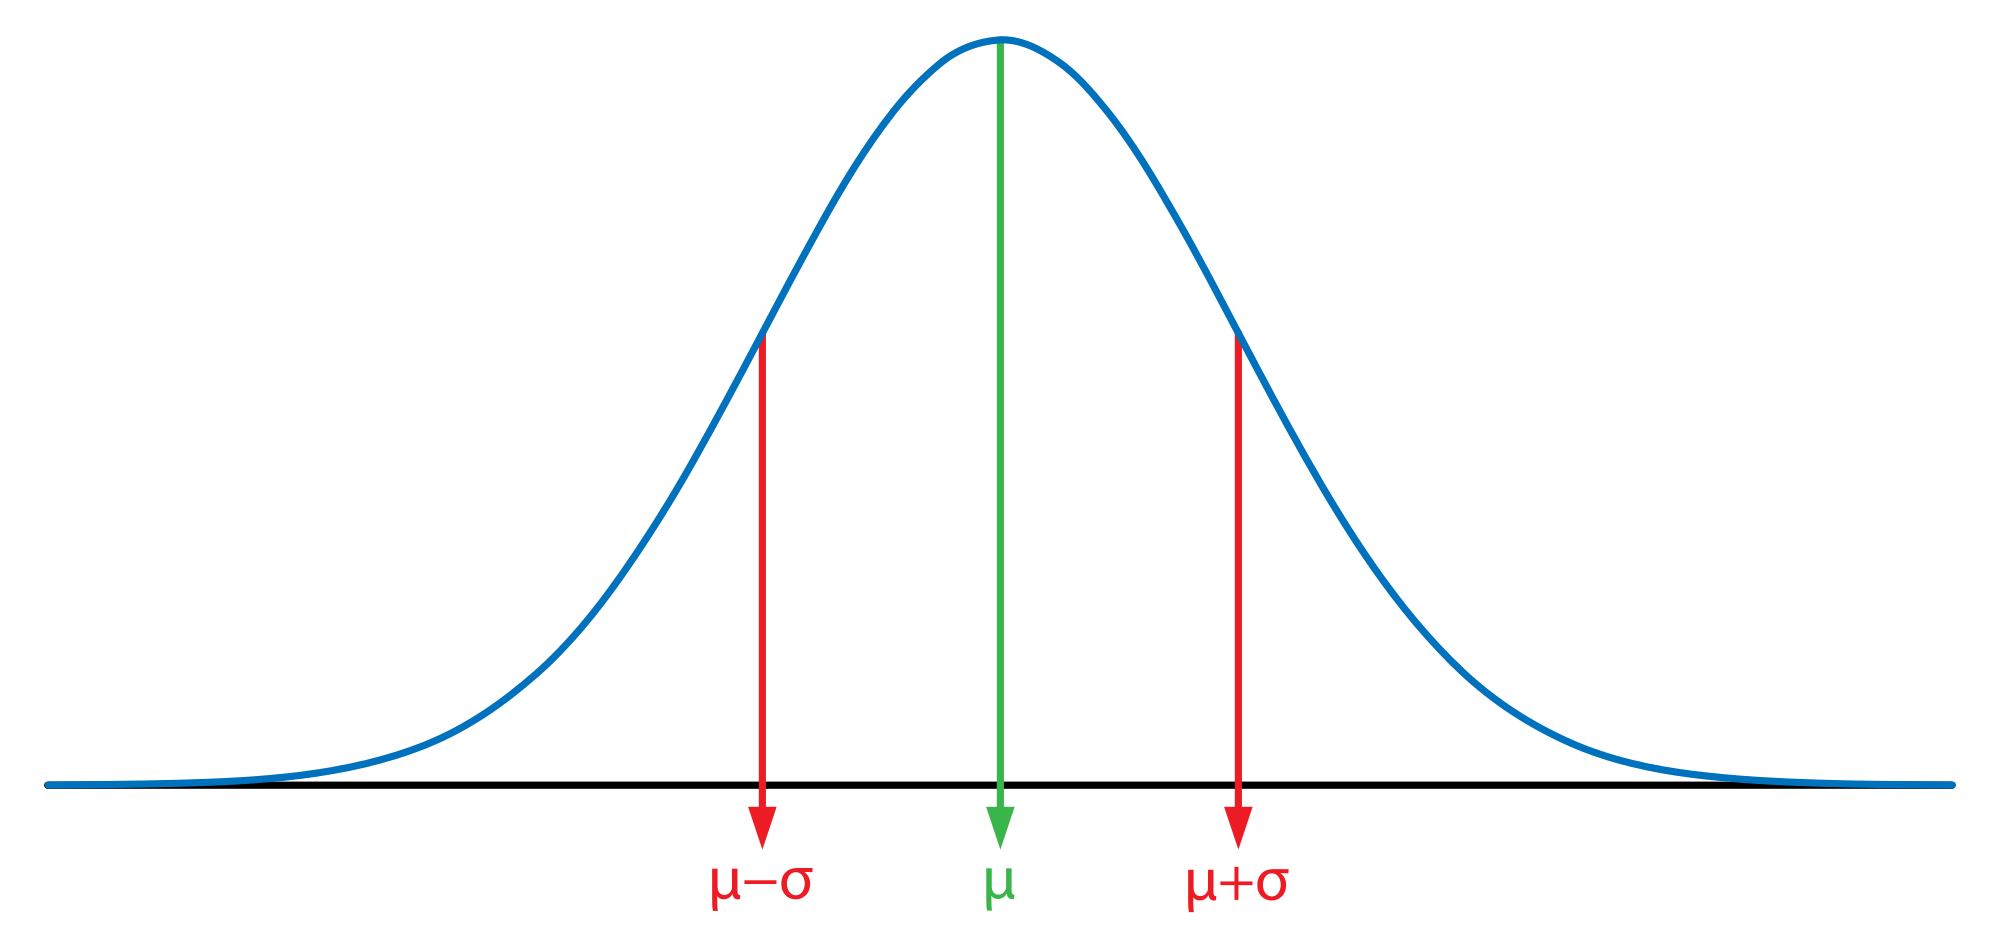
\includegraphics[width=.5\linewidth]{graphics/normal-distribution.png}
          \end{figure}
      \item<5-> $W$ has continuous trajectories.
    \end{enumerate}
  \end{definition}
  \end{onlyenv}
  \begin{onlyenv}<6->
    \begin{theorem}
      A Wiener trajectory is with probability one, nowhere differentiable, and it has locally infinite total variation.
    \end{theorem}
    \begin{figure}
      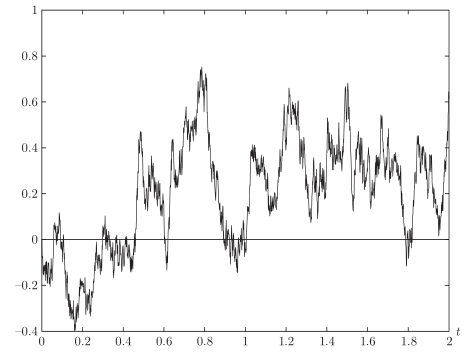
\includegraphics[scale=.45]{./graphics/wiener-trajectory.png}
      \caption{Wiener trajectory}
    \end{figure}
  \end{onlyenv}
\end{frame}

\begin{frame}[t]
  \frametitle{Quadratic Variation}
  \begin{onlyenv}<1->
    \begin{definition}
      Let $X$ be a stochastic process. Suppose $P$ is a partition of $[0,t]$ denoted $t_k$ and let $\lVert P \rVert$ be the mesh of the partition then the \textbf{quadratic variation} of $X$ is defined to be:
          \begin{align*}
            [X]_t = \lim\limits_{\lVert P \rVert \to 0} \displaystyle\sum_{k = 1}^{n}(X_{t_k} - X_{t_{k-1}})^2.
          \end{align*}
    \end{definition}
  \end{onlyenv}
  \begin{onlyenv}<2->
    \begin{block}{Comments}
      Note that Quadratic Variation itself is a stochastic process. An intuitive way to think about quadratic variation is the internal clock of a process, describing how randomness accumulates over time.
    \end{block}
  \end{onlyenv}
\end{frame}



\begin{frame}[t]
  \frametitle{Quadratic Variation of Wiener Process}
    \begin{onlyenv}<1-3>
    \begin{theorem}
      Quadratic variation of a Wiener Process on the interval $[0,t]$ is $t$.
    \end{theorem}
    \end{onlyenv}
    \begin{onlyenv}<2-3>
      \begin{block}{Proof.}
        Let $P = \{0 = t_0 \leq t_1 \leq \dots \leq t_m = t\}$ be a partition of the interval $[0,t]$. Then the quadratic variation on $P$ is:
        \begin{align*}
          [W]^{P}_{t} &= \displaystyle\sum_{k = 1}^{m}(W_{t_k} - W_{t_{k-1}})^2 .
        \end{align*}
        \onslide<3->{
          Therefore,
          \begin{align*}
            \mathbb{E}\left[[W]^{P}_{t}\right] &= \displaystyle\sum_{k = 1}^{m}\mathbb{E}\left[(W_{t_k} - W_{t_{k-1}})^2\right].
          \end{align*}
        }
      \end{block}
    \end{onlyenv}
    \begin{onlyenv}<4>
        \begin{theorem}
          \begin{align*}
            Var(X) = \mathbb{E}(X^2) - (\mathbb{E}(X))^2.
          \end{align*}
        \end{theorem}
    \end{onlyenv}
    \begin{onlyenv}<5-8>
      \begin{block}{Proof cont.}
        Since $W_{t_{k}} - W_{t_{k-1}} \in \mathcal{N}(0, t_{k} - t_{k-1})$, 
        \begin{align*}
          \mathbb{E}(W_{t_{k}} - W_{t_{k-1}}) = 0.
        \end{align*}
        \onslide<6->{ 
          It follows that:
          \begin{align*}
            (\mathbb{E}\left[W_{t_{k}} - W_{t_{k-1}}\right])^2 = 0 .
          \end{align*}
        }
        \onslide<7->{
          Thus, $Var(W_{t_{k}} - W_{t_{k-1}}) = E(\left[W_{t_{k}} - W_{t_{k-1}}\right]^2)$.
        }
        \onslide<8->{%
          \begin{block}{}
            Since $\mathbb{E}[(W_{t_{k}} - W_{t_{k-1}})^2] = Var\left[W_{t_{k}} - W_{t_{k-1}}]$, we can write:
            \begin{align*}
              \mathbb{E}\left[[W]^{P}_{t}\right] &= \mathbb{E}\left[ \displaystyle\sum_{k = 1}^{m}(W_{t_k} - W_{t_{k-1}})^2 \right] = Var \left[\displaystyle\sum_{k = 1}^{m}\left[ W_{t_k} - W_{t_{k-1}} \right] \right]. \\
            \end{align*}
          \end{block}
        }
      \end{block}
    \end{onlyenv}
    \begin{onlyenv}<9>
      \begin{block}{Stats fact}
      \begin{align*}
        Var \left[\displaystyle\sum_{k = 1}^{m}\left[ W_{t_k} - W_{t_{k-1}} \right] \right] &= \displaystyle\sum_{k = 1}^{m}Var\left[ W_{t_k} - W_{t_{k-1}} \right] \\ 
        &+ \displaystyle\sum_{k \neq \ell}^{m}Cov\left(\left[ W_{t_k} - W_{t_{k-1}} \right], \left[ W_{t_{\ell}} - W_{t_{\ell-1}} \right]\right)
      \end{align*}
      \end{block}
    \end{onlyenv}
    \begin{onlyenv}<10-13>
      \begin{block}{Proof cont.}
      \onslide<10->{%
        Since Wiener increments are independent of eachother, 
        \begin{align*}
          Cov\left(\left[ W_{t_k} - W_{t_{k-1}} \right], \left[ W_{t_{\ell}} - W_{t_{\ell-1}} \right]\right) = 0.
        \end{align*}
      }
      \onslide<11->{%
      Therefore, 
      \begin{align*}
        E\left[ \left[ W \right]^{P}_{t}] \right] = \displaystyle\sum_{k = 1}^{m}Var\left[ W_{t_{k}} - W_{t_{k-1}} \right]
      \end{align*}
      }
      \onslide<12->{%
        Using $W_{t_k} - W_{t_{k-1}} \in \mathcal{N}(0, t_k - t_{k-1})$:
        \begin{align*}
          \mathbb{E}\left[[W]^{P}_{t}\right] &= \displaystyle\sum_{k = 1}^{m}(t_{k} - t_{k-1}) \\
          &= t
        \end{align*}
      }
      \onslide<13->{% 
        Now we must show $\mathbb{E}([W]^{P}_{t}) = [W]_t = t$.
      }
      \end{block}
    \end{onlyenv}
    \begin{onlyenv}<14>
      \begin{block}{Stats fact}
        If $Var(X) = 0$ then $X = \mathbb{E}\left[ X \right]$.
      \end{block}
    \end{onlyenv}
    \begin{onlyenv}<15-16>
      \begin{block}{Proof.}
        Let us fix a point $t$ and subdivide the interval $[0,t]$ into $n$ equally large subintervals of the form $[k\frac{t}{n}, (k+1)\frac{t}{n}]$, where $k = 0,1,\ldots,n-1$. These subintervals will be our partition $P$. Therefore, we must show that :
        \begin{align*}
          Var(\lim\limits_{\Vert P \Vert \to 0} \left[ W \right]^{P}_t) = 0.
        \end{align*}
        Or equivalently,
        \begin{align*}
          Var(\lim\limits_{n \to \infty} \displaystyle\sum_{i=1}^{n}\left[W_{i(\frac{t}{n})} - W_{(i-1)(\frac{t}{n})}\right]^2) = 0,
        \end{align*}
        \onslide<16->{
        and we showed earlier:
        \begin{align*}
          Var(\lim\limits_{n \to \infty} \displaystyle\sum_{i=1}^{n}\left[W_{i(\frac{t}{n})} - W_{(i-1)(\frac{t}{n})}\right]^2) = \lim\limits_{n \to \infty} \displaystyle\sum_{i=1}^{n} Var(\left[W_{i(\frac{t}{n})} - W_{(i-1)(\frac{t}{n})}\right]^2).
        \end{align*}
        }
      \end{block}
    \end{onlyenv}
    \begin{onlyenv}<17,19>
      \begin{block}{Proof.}
        Also from earlier:
        \begin{align*}
          Var(\lim\limits_{n \to \infty} \displaystyle\sum_{i=1}^{n}\left[W_{i(\frac{t}{n})} - W_{(i-1)(\frac{t}{n})}\right]^2) &= \lim\limits_{n \to \infty} \displaystyle\sum_{i=1}^{n} \mathbb{E}(\left[W_{i(\frac{t}{n})} - W_{(i-1)(\frac{t}{n})}\right]^4) \\
          &- \mathbb{E}\left(\left[W_{i(\frac{t}{n})} - W_{(i-1)(\frac{t}{n})}\right]^2\right)^2.
        \end{align*}
        \onslide<19->{ 
        Therefore,
        \begin{align*}
          Var(\lim\limits_{n \to \infty} \displaystyle\sum_{i=1}^{n}\left[W_{i(\frac{t}{n})} - W_{(i-1)(\frac{t}{n})}\right]^2) &= \lim\limits_{n \to \infty} \displaystyle\sum_{i=1}^{n} 3\left(i(\frac{t}{n}) - (i-1)(\frac{t}{n})\right)^2 \\ 
          &- \left(i(\frac{t}{n}) - (i-1)(\frac{t}{n})\right)^2.
        \end{align*}
        }
      \end{block}
    \end{onlyenv}
    \begin{onlyenv}<18>
      \begin{block}{Stats fact}
        \mathbb{E}\left[\left(X - \mu \right)^p \right] = \begin{cases}
          0, &\text{ if }p \text{ is odd}\\
          \sigma^p(p - 1)!!, &\text{ if }p \text{ is even}.
        \end{cases}
      \end{block}
    \end{onlyenv}
    \begin{onlyenv}<20-21>
      \begin{block}{Proof.}
        Simplifying,
        \begin{align*}
          Var(\lim\limits_{n \to \infty} \displaystyle\sum_{i=1}^{n}\left[W_{i(\frac{t}{n})} - W_{(i-1)(\frac{t}{n})}\right]^2) &= \lim\limits_{n \to \infty} \displaystyle\sum_{i=1}^{n} 2\frac{t^2}{n^2}, \\
          &= \lim\limits_{n \to \infty} 2\frac{t^2}{n}, \\
          &= 0.
        \end{align*}
        \onslide<21->{ 
        Thus,
        \begin{align*}
          \left[ W \right]_t = \mathbb{E}\left( \left[ W \right]_t \right) = \mathbb{E}\left( \lim\limits_{\Vert P \Vert \to 0} \left[ W \right]^{P}_{t} \right).
        \end{align*}
        }
      \end{block}
    \end{onlyenv}
    \begin{onlyenv}<22-23>
      \begin{proof}
        By dominating convergence theorem (outside scope),
        \begin{align*}
          \mathbb{E}\left( \lim\limits_{\Vert P \Vert \to 0} \left[ W \right]^{P}_{t} \right) &= \lim\limits_{\Vert P \Vert \to 0},
          \mathbb{E}\left(\left[ W \right]^{P}_{t} \right), \\
          &= \lim\limits_{\Vert P \Vert \to 0} t, \\
          &= t.
        \end{align*}
        \onslide<23>{ 
        Thus, $\left[ W \right]_t = t$.
        }
      \end{proof}
    \end{onlyenv}
    \begin{onlyenv}<24>
      \begin{block}{Implications}
        This motivates us to write:
        \begin{align*}
          \int\limits_{0}^{t}(dW_t)^2 = t.
        \end{align*}
        Or equivalently,
        \begin{align*}
          (dW_t)^2 = dt.
        \end{align*}
        This will come up frequently later as we transitition into Ito calculus.
      \end{block}
  \end{onlyenv}
\end{frame}

\begin{frame}[t]
  \frametitle{The Stochastic Integral}
  \begin{onlyenv}<1>
    \begin{block}{Motivation}
      Let $h_t$ be a stochastic process that represents our trading strategy and let $W_t$ be the price of the stock at the given time. Then
      \begin{align*}
        \displaystyle\int_{0}^{t} h_t dW_t
      \end{align*}
      would be our gains or losses from this strategy.
    \end{block}
  \end{onlyenv}
  \begin{onlyenv}<2-4>
    \begin{block}{The Problem}
      Integrals of the form $\displaystyle\int_{0}^{t}g_s dW_s$ for some stochastic process $g_s$.
    \end{block}
  \end{onlyenv}
  \begin{onlyenv}<3-4>
    \begin{block}{Possible Solution 1}
      Try to define like the Riemman Integral:
      \begin{enumerate}
        \item<3-> $\displaystyle\sum_{k = 1}^{n}g_s(W_{t_{k+1}} - W_{t_{k}})$,
        \item<4-> Not possible due to locally unbounded variation of a Wiener Process.
      \end{enumerate}
    \end{block}
  \end{onlyenv}
  \begin{onlyenv}<5-6>
    \begin{definition}
      A stochastic process is \textbf{simple} on $[a,b]$ when there exists deterministic points in time $a = t_0 < t_1 < \dots < t_n = b$ such that $g_s = g_{t_k}$ for all $s \in [t_k, t_{k+1}]$.
    \end{definition}
  \end{onlyenv}
  \begin{onlyenv}<6>
      \begin{block}{Real Solution}
        Now we can define the stochastic integral by
        \begin{align*}
          \displaystyle\int_{a}^{b}g_s dW_s = \displaystyle\sum_{k = 0}^{n - 1}g_{t_k}[W_{t_{k+1}} - W_{t_{k}}],
        \end{align*}
        for some simple stochastic process $g_s$.
      \end{block}
  \end{onlyenv}
  \begin{onlyenv}<7->
    \begin{block}{Generalized Version}
      By the \textbf{simple approximation theorem} (outside of scope), for some stochastic process $g_s$ there exists a sequence of simple functions $g_{s}^{n}$, such that $g_{s}^{n} \to g_{s}$. Therefore, we define our integral for non-simple functions as:
      \begin{align*}
        \displaystyle\int_{a}^{b}g_{s} dW_t = \lim\limits_{n \to \infty}\displaystyle\int_{a}^{b} g_{s}^{n}dW_t.
      \end{align*}
    \end{block}
    \onslide<8->{ 
    \begin{block}{Something to think about}
      How might we evaluate $\displaystyle\int_{0}^{t} W_s dW_s$?
    \end{block}
    }
  \end{onlyenv}
\end{frame}

\begin{frame}[t]
  \frametitle{Stochastic Differential Equations}
  \begin{definition}
    An ito process, $X_t$, is a process that can be represented as:
    \begin{align*}
      X_t = X_0 + \displaystyle\int_{0}^{t}\mu_s ds + \displaystyle\int_{0}^{t}\sigma_s dW_s.
    \end{align*}
  \end{definition}
  \onslide<2->{ 
  We often use the notation:
  \begin{align*}
    dX_t = \mu_t dt + \sigma_t dW_t.
  \end{align*}
  }
  \onslide<3->{ 
  This is known as a stochastic differential equation, and a useful tool for solving these is Ito's lemma, which we will see shortly.
  }
\end{frame}

\begin{frame}[t]
  \frametitle{Ito's Multiplication Table}
  \begin{onlyenv}<1-2>
  \begin{definition}
    \textbf{Ito's multiplication table} is: 
    \begin{center}
      \renewcommand\arraystretch{1.3}
      \setlength\doublerulesep{0pt}
      \begin{tabular}{r||*{4}{2|}}
       & $dt$ & $dW_t$ \\
      \hline\hline
      $dt$ & 0 & 0 \\ 
      \hline
      $dW_t$ & 0 & $dt$ \\ 
      \end{tabular}
    \end{center}
    \end{definition}
    We have already shown the only interesting result: $(dW_t)^2 = dt$.
  \end{onlyenv}
  \begin{onlyenv}<2>
    \begin{proof}[Quick sketch.]
      Suppose you are integrating on the interval $[a,b]$. Partition [a,b] into $N$ increments. Then $dt \sim \frac{1}{N}$ and $(dt)^2 \sim \frac{1}{N^2}$. It follows that:
      \begin{align*}
        \displaystyle\sum_{i = 1}^{N}\frac{1}{N^2} &= \frac{1}{N}, \\
        \lim\limits_{N \to \infty}\displaystyle\sum_{i = 1}^{N}\frac{1}{N^2} &= \lim\limits_{N \to \infty} \frac{1}{N} = \displaystyle\int_{a}^{b}(dt)^2 = 0.
      \end{align*}
    \end{proof}
  \end{onlyenv}
  \begin{onlyenv}<3->
    \begin{proof}[Quick sketch.]
      Similarly, suppose you are integrating on the interval $[a,b]$. Partition [a,b] into $N$ increments. Since $dW_t = \sqrt{dt}$, $dt \sim \frac{1}{N}$ and $(dt) (dW_t) \sim \frac{1}{N^{3/2}}$. It follows that:
      \begin{align*}
        \displaystyle\sum_{i = 1}^{N}\frac{1}{N^{3/2}} &= \frac{1}{N^{1/2}}, \\
        \lim\limits_{N \to \infty}\displaystyle\sum_{i = 1}^{N}\frac{1}{N^{3/2}} &= \lim\limits_{N \to \infty} \frac{1}{N^{1/2}} = \displaystyle\int_{a}^{b}(dt)(dW_t) = 0.
      \end{align*}
    \end{proof}
  \end{onlyenv}
  \begin{onlyenv}<4->
    This completes the multiplication table and provides the foundation for introducing Ito's lemma.
  \end{onlyenv}
\end{frame}

\begin{frame}[t]
  \frametitle{Ito's Lemma}
  \begin{onlyenv}<1>
  \begin{theorem}[Ito's formula]
    Assume that process $X$ has a stochastic differential given by 
    \begin{align*}
      dX_t = \mu_t dt + \sigma_t dW_t.
    \end{align*}
    Define the process $Z$ by $Z(t) = f(t, X_t)$. Then $Z$ has a stochastic differential given by
    \begin{align*}
      df(t, X_t) &= \left\{\frac{\partial f}{\partial t}(t, X_t) + \mu_t \frac{\partial f}{\partial x}(t,X_t) + \frac{1}{2}\sigma^2_t\frac{\partial^2 f}{\partial x^2}(t,X_t)\right\}dt + \sigma \frac{\partial f}{\partial x}(t, X_t)dW_t.
    \end{align*}
  \end{theorem}
  \end{onlyenv}
  \begin{onlyenv}<2-5>
    \begin{block}{Heuristic proof.}
      Using $f$ from the theorem, we will consider the second order Taylor expansion:
      \begin{align*}
        df = \frac{\partial f}{\partial t}dt + \frac{\partial f}{\partial x}dX_t + \frac{1}{2}\frac{\partial^2 f}{\partial x ^2}(dX_t)^2 + \frac{1}{2}\frac{\partial^2 f}{\partial t^2}(dt)^2 + \frac{\partial^2 f}{\partial t \partial x}dt dX_t.
      \end{align*}
      \onslide<3-5>{
      By definition we have:
      \begin{align*}
        dX_t = \mu_t dt + \sigma_t dW_t.
      \end{align*}
      }
      \onslide<4-5>{
      so, we obtain
      \begin{align*}
        (dX_t)^2 = \mu^2_t(dt)^2 + 2\mu_t \sigma_t(dt)(dW_t) + \sigma^2_t(dW_t)^2.
      \end{align*}
      }
      \onslide<5>{
      From Ito's multiplication table we have:
      \begin{align*}
        (dX_t)^2 = \sigma^2_t dt.
      \end{align*}
      }
    \end{block}
  \end{onlyenv}
  \begin{onlyenv}<6-8>
    \begin{proof}[Heuristic proof cont.]
      Substituting back for $(dX_t)^2$,
      \begin{align*}
        df = \frac{\partial f}{\partial t}dt + \frac{\partial f}{\partial x}dX_t + \frac{1}{2}\frac{\partial^2 f}{\partial x ^2}(\sigma^2_t)(dt) + \frac{1}{2}\frac{\partial^2 f}{\partial t^2}(dt)^2 + \frac{\partial^2 f}{\partial t \partial x}dt dX_t.
      \end{align*}
    \onslide<7->{
      Applying Ito's multiplication table one more time,
      \begin{align*}
        df = \frac{\partial f}{\partial t}dt + \frac{\partial f}{\partial x}dX_t + \frac{1}{2}\frac{\partial^2 f}{\partial x ^2}(\sigma^2_t)(dt) + \frac{\partial^2 f}{\partial t \partial x}dt dX_t.
      \end{align*}
    }
    \onslide<8->{
      Now substituing in $(dX_t)$,
      \begin{align*}
        df &= \frac{\partial f}{\partial t}dt + \frac{\partial f}{\partial x}(\mu_t dt + \sigma_t dW_t) + \frac{1}{2}\frac{\partial^2 f}{\partial x ^2}(\sigma^2_t)(dt) + \frac{\partial^2 f}{\partial t \partial x}(\mu_t dt + \sigma_t dW_t)dt, \\
        &= \left\{\frac{\partial f}{\partial t}(t, X_t) + \mu_t \frac{\partial f}{\partial x}(t,X_t) + \frac{1}{2}\sigma^2_t\frac{\partial^2 f}{\partial x^2}(t,X_t)\right\}dt + \sigma \frac{\partial f}{\partial x}(t, X_t)dW_t.
      \end{align*}
    }
    \end{proof}
  \end{onlyenv}
  \begin{onlyenv}<9-12>
    \begin{example}
      Find $d(W_{t}^2)$.
    \end{example}
  \end{onlyenv}
  \begin{onlyenv}<10-12>
    \begin{solution}
      Define $X$ by $X_t = W_t$ and set $f(t,x) = x^2$. In terms of Ito's formula we have
      \begin{align*}
        \frac{\partial f}{\partial t}(t,x) = 0,\ \frac{\partial f}{\partial x}(t,x) = 2x,\ \frac{\partial^2 f}{\partial t^2}(t,x) = 2.
      \end{align*}
      \onslide<11->{
      Substituting,
      \begin{align*}
        d(W_{t}^2) = \left\{0 + 0 \cdot 2X_t + \frac{1}{2}\cdot 1 \cdot 2 \right\}dt + 1 \cdot 2X_t dW_t.
      \end{align*}
      }
      \onslide<12->{
      Thus,
      \begin{align*}
        d(W_t^2) = dt + 2W_t dW_t.
      \end{align*}
      }
    \end{solution}
  \end{onlyenv}
  \begin{onlyenv}<13->
    \begin{block}{Revisiting}
      Now if we integrate both side such that:
      \begin{align*}
        \displaystyle\int_{0}^{t} d(W_t^2) = \displaystyle\int_{0}^{t}dt + \displaystyle\int_{0}^{t}2W_t dW_t. \\
      \end{align*}
      \onslide<14->{
      This gives us:
      \begin{align*}
        \displaystyle\int_{0}^{t}W_t dW_t = \frac{W_t^2}{2} - \frac{t}{2}.
      \end{align*}
      }
    \end{block}
  \end{onlyenv}
\end{frame}

\begin{frame}[t]
  \frametitle{Real world application}
  \begin{onlyenv}<1-2>
    \begin{definition}
      \textbf{Geometric Brownian Motion} is a stochastic process whose dynamics follow the stochastic differential equation 
      \begin{align*}
        dX_t = \alpha X_t dt + \sigma X_t dW_t \text{ for some } \alpha,\beta \in \mathbb{R},
      \end{align*}
      where $dW_t$ is the infinitesimal increment of the Wiener process.
    \end{definition}
    \onslide<2->{
      \begin{block}{}
        Geometric Brownian Motion is one of the building blocks for the modeling of asset prices, and turns up naturally in many other places.
      \end{block}
    }
  \end{onlyenv}
  \begin{onlyenv}<3-4>
    \begin{block}{Closed form}
      With our toolbox of Ito calculus and the ability to solve linear ODE's, it can be easily shown that the closed form of Geometric Brownian Motion is:
      \begin{align*}
        dX_t = X_0 e^{(\mu - \frac{\sigma^2}{2})dt + \sigma dW_t}.
      \end{align*}
    \end{block}
    \onslide<4->{ 
    Now let's see how accurate this elementary model is when trying to predict the price of real stocks.
    }
  \end{onlyenv}
  \begin{onlyenv}<5-6>
    \begin{block}{Use in Finance}
      Black Scholes Model is one of the most widely used models of stock price behaviour and is built on Geometric Brownian motion.
    \end{block}
    \begin{block}{Why GBM?}
      Some of the arguments for GBM are:
      \begin{itemize}
        \item<6-> The expected returns are independent of the value of the process, which is how stocks behave in reality,
      \end{itemize}
    \end{block}
  \end{onlyenv}
  \begin{onlyenv}<7>
    \begin{block}{Simulation}
      Ten iterations based off Facebook closing price in the past year:
      \begin{figure}
        \centering
        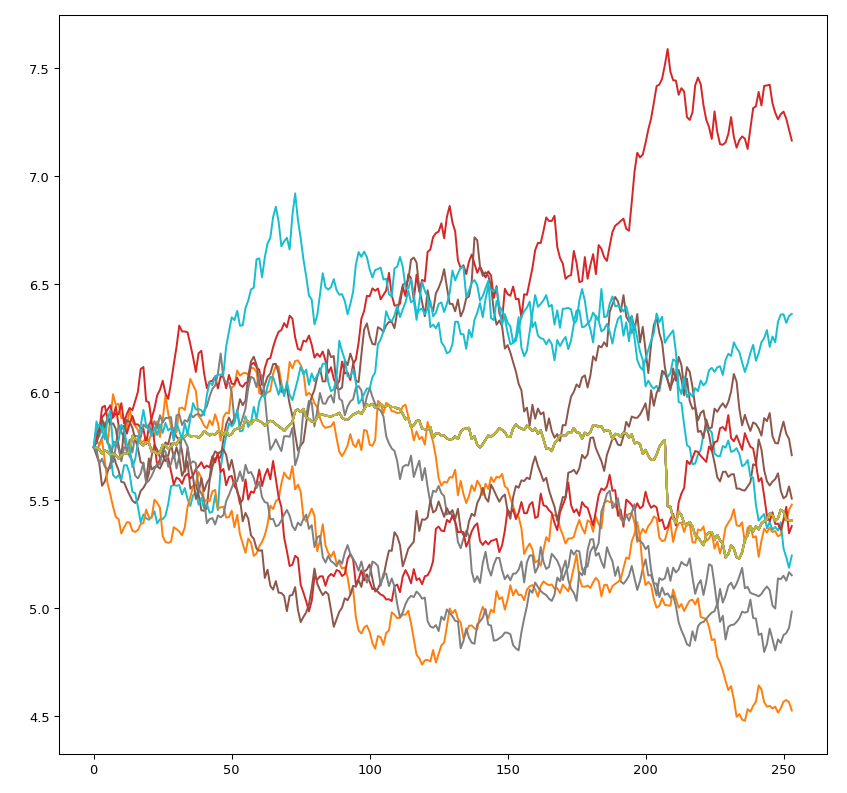
\includegraphics[width=.5\linewidth]{graphics/monte-carlo.png}
      \end{figure}
    \end{block}
  \end{onlyenv}
\end{frame}
\end{document}
